% GNUPLOT: LaTeX picture with Postscript
\begingroup
  \makeatletter
  \providecommand\color[2][]{%
    \GenericError{(gnuplot) \space\space\space\@spaces}{%
      Package color not loaded in conjunction with
      terminal option `colourtext'%
    }{See the gnuplot documentation for explanation.%
    }{Either use 'blacktext' in gnuplot or load the package
      color.sty in LaTeX.}%
    \renewcommand\color[2][]{}%
  }%
  \providecommand\includegraphics[2][]{%
    \GenericError{(gnuplot) \space\space\space\@spaces}{%
      Package graphicx or graphics not loaded%
    }{See the gnuplot documentation for explanation.%
    }{The gnuplot epslatex terminal needs graphicx.sty or graphics.sty.}%
    \renewcommand\includegraphics[2][]{}%
  }%
  \providecommand\rotatebox[2]{#2}%
  \@ifundefined{ifGPcolor}{%
    \newif\ifGPcolor
    \GPcolortrue
  }{}%
  \@ifundefined{ifGPblacktext}{%
    \newif\ifGPblacktext
    \GPblacktexttrue
  }{}%
  % define a \g@addto@macro without @ in the name:
  \let\gplgaddtomacro\g@addto@macro
  % define empty templates for all commands taking text:
  \gdef\gplbacktext{}%
  \gdef\gplfronttext{}%
  \makeatother
  \ifGPblacktext
    % no textcolor at all
    \def\colorrgb#1{}%
    \def\colorgray#1{}%
  \else
    % gray or color?
    \ifGPcolor
      \def\colorrgb#1{\color[rgb]{#1}}%
      \def\colorgray#1{\color[gray]{#1}}%
      \expandafter\def\csname LTw\endcsname{\color{white}}%
      \expandafter\def\csname LTb\endcsname{\color{black}}%
      \expandafter\def\csname LTa\endcsname{\color{black}}%
      \expandafter\def\csname LT0\endcsname{\color[rgb]{1,0,0}}%
      \expandafter\def\csname LT1\endcsname{\color[rgb]{0,1,0}}%
      \expandafter\def\csname LT2\endcsname{\color[rgb]{0,0,1}}%
      \expandafter\def\csname LT3\endcsname{\color[rgb]{1,0,1}}%
      \expandafter\def\csname LT4\endcsname{\color[rgb]{0,1,1}}%
      \expandafter\def\csname LT5\endcsname{\color[rgb]{1,1,0}}%
      \expandafter\def\csname LT6\endcsname{\color[rgb]{0,0,0}}%
      \expandafter\def\csname LT7\endcsname{\color[rgb]{1,0.3,0}}%
      \expandafter\def\csname LT8\endcsname{\color[rgb]{0.5,0.5,0.5}}%
    \else
      % gray
      \def\colorrgb#1{\color{black}}%
      \def\colorgray#1{\color[gray]{#1}}%
      \expandafter\def\csname LTw\endcsname{\color{white}}%
      \expandafter\def\csname LTb\endcsname{\color{black}}%
      \expandafter\def\csname LTa\endcsname{\color{black}}%
      \expandafter\def\csname LT0\endcsname{\color{black}}%
      \expandafter\def\csname LT1\endcsname{\color{black}}%
      \expandafter\def\csname LT2\endcsname{\color{black}}%
      \expandafter\def\csname LT3\endcsname{\color{black}}%
      \expandafter\def\csname LT4\endcsname{\color{black}}%
      \expandafter\def\csname LT5\endcsname{\color{black}}%
      \expandafter\def\csname LT6\endcsname{\color{black}}%
      \expandafter\def\csname LT7\endcsname{\color{black}}%
      \expandafter\def\csname LT8\endcsname{\color{black}}%
    \fi
  \fi
    \setlength{\unitlength}{0.0500bp}%
    \ifx\gptboxheight\undefined%
      \newlength{\gptboxheight}%
      \newlength{\gptboxwidth}%
      \newsavebox{\gptboxtext}%
    \fi%
    \setlength{\fboxrule}{0.5pt}%
    \setlength{\fboxsep}{1pt}%
\begin{picture}(11520.00,5760.00)%
    \gplgaddtomacro\gplbacktext{%
      \csname LTb\endcsname%
      \put(1229,1371){\makebox(0,0)[r]{\strut{}0.000010}}%
      \csname LTb\endcsname%
      \put(1229,2093){\makebox(0,0)[r]{\strut{}0.000100}}%
      \csname LTb\endcsname%
      \put(1229,2816){\makebox(0,0)[r]{\strut{}0.001000}}%
      \csname LTb\endcsname%
      \put(1229,3538){\makebox(0,0)[r]{\strut{}0.010000}}%
      \csname LTb\endcsname%
      \put(1229,4261){\makebox(0,0)[r]{\strut{}0.100000}}%
      \csname LTb\endcsname%
      \put(1229,4983){\makebox(0,0)[r]{\strut{}1.000000}}%
      \csname LTb\endcsname%
      \put(1331,967){\makebox(0,0){\strut{}$10$}}%
      \csname LTb\endcsname%
      \put(2006,967){\makebox(0,0){\strut{}$100$}}%
      \csname LTb\endcsname%
      \put(2680,967){\makebox(0,0){\strut{}$1000$}}%
      \csname LTb\endcsname%
      \put(3355,967){\makebox(0,0){\strut{}$10000$}}%
      \csname LTb\endcsname%
      \put(4030,967){\makebox(0,0){\strut{}$100000$}}%
      \csname LTb\endcsname%
      \put(4704,967){\makebox(0,0){\strut{}$1\times10^{6}$}}%
      \csname LTb\endcsname%
      \put(5379,967){\makebox(0,0){\strut{}$1\times10^{7}$}}%
    }%
    \gplgaddtomacro\gplfronttext{%
      \csname LTb\endcsname%
      \put(218,3177){\rotatebox{-270}{\makebox(0,0){\strut{}Error}}}%
      \csname LTb\endcsname%
      \put(3355,688){\makebox(0,0){\strut{}N}}%
      \csname LTb\endcsname%
      \put(3355,5480){\makebox(0,0){\strut{}Error}}%
      \csname LTb\endcsname%
      \put(2669,539){\makebox(0,0)[r]{\strut{}Plain}}%
      \csname LTb\endcsname%
      \put(2669,353){\makebox(0,0)[r]{\strut{}Halton}}%
      \csname LTb\endcsname%
      \put(2669,167){\makebox(0,0)[r]{\strut{}Lattice}}%
      \csname LTb\endcsname%
      \put(4579,539){\makebox(0,0)[r]{\strut{}FitP :a:{0.57}}}%
      \csname LTb\endcsname%
      \put(4579,353){\makebox(0,0)[r]{\strut{}FitH :a:{0.99}}}%
      \csname LTb\endcsname%
      \put(4579,167){\makebox(0,0)[r]{\strut{}FitL :a:{0.96}}}%
    }%
    \gplgaddtomacro\gplbacktext{%
      \csname LTb\endcsname%
      \put(6915,1118){\makebox(0,0)[r]{\strut{}0.000010}}%
      \csname LTb\endcsname%
      \put(6915,1867){\makebox(0,0)[r]{\strut{}0.000100}}%
      \csname LTb\endcsname%
      \put(6915,2616){\makebox(0,0)[r]{\strut{}0.001000}}%
      \csname LTb\endcsname%
      \put(6915,3366){\makebox(0,0)[r]{\strut{}0.010000}}%
      \csname LTb\endcsname%
      \put(6915,4115){\makebox(0,0)[r]{\strut{}0.100000}}%
      \csname LTb\endcsname%
      \put(6915,4864){\makebox(0,0)[r]{\strut{}1.000000}}%
      \csname LTb\endcsname%
      \put(7017,707){\makebox(0,0){\strut{}$10$}}%
      \csname LTb\endcsname%
      \put(7716,707){\makebox(0,0){\strut{}$100$}}%
      \csname LTb\endcsname%
      \put(8416,707){\makebox(0,0){\strut{}$1000$}}%
      \csname LTb\endcsname%
      \put(9115,707){\makebox(0,0){\strut{}$10000$}}%
      \csname LTb\endcsname%
      \put(9814,707){\makebox(0,0){\strut{}$100000$}}%
      \csname LTb\endcsname%
      \put(10514,707){\makebox(0,0){\strut{}$1\times10^{6}$}}%
      \csname LTb\endcsname%
      \put(11213,707){\makebox(0,0){\strut{}$1\times10^{7}$}}%
    }%
    \gplgaddtomacro\gplfronttext{%
      \csname LTb\endcsname%
      \put(5904,2991){\rotatebox{-270}{\makebox(0,0){\strut{}Error}}}%
      \csname LTb\endcsname%
      \put(9115,428){\makebox(0,0){\strut{}N}}%
      \csname LTb\endcsname%
      \put(9115,5368){\makebox(0,0){\strut{}Estimated Error }}%
      \csname LTb\endcsname%
      \put(7729,167){\makebox(0,0)[r]{\strut{}Plain}}%
      \csname LTb\endcsname%
      \put(9129,167){\makebox(0,0)[r]{\strut{}Halton}}%
      \csname LTb\endcsname%
      \put(10529,167){\makebox(0,0)[r]{\strut{}Lattice}}%
    }%
    \gplbacktext
    \put(0,0){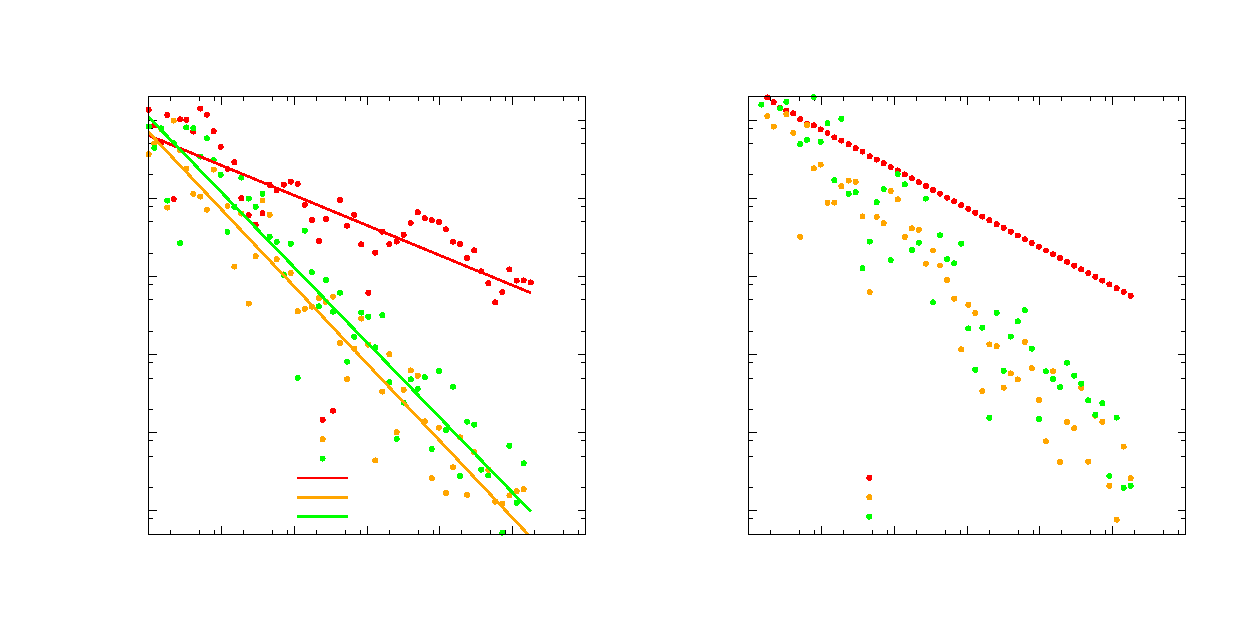
\includegraphics{plotSin}}%
    \gplfronttext
  \end{picture}%
\endgroup
